\documentclass[13pt]{article}
\usepackage[utf8]{inputenc}

\title{Exercise 3: Topic 3.4\\ Generation and Evaluation of Unstructured Synthetic Datasets}
\author{Rafael Sterzinger, Christian Stippel, Fatjon Zogaj}
\date{January 31, 2020}

\usepackage{graphicx,wrapfig,lipsum}
\usepackage{animate}
\usepackage{graphicx}
\usepackage{subcaption}
\usepackage{cleveref}
\setlength{\parindent}{0pt}
\usepackage[margin=1.2in]{geometry}
\setlength{\parskip}{1em}

\begin{document}

\maketitle

\section{Introduction} \label{sec:introduction}
For our third and last exercise in Machine Learning, we have decided to take on the experimental problem of generating unstructured synthetic datasets using a Generative Adversarial Network (GAN) as well as evaluating and comparing the classification accuracy when training a Convolutional Neural Network (CNN) with the generated data.

We have trained three CNNs to classify on the following kinds of data:
\begin{itemize}
    \item original training data
    \item augmented training data
    \item synthetically generated data
\end{itemize}

Afterwards we compared their classification performance in regards to the original validation data. We have expanded on the exercise's assignment, by including data augmentation, created by flipping, zooming, rotating and changing the brightness level of the original training data. Comparing synthetic generated data to data augmentation is necessary, since both approaches seem to tackle the similar problem of a too small training set.
We have constructed our analysis on the following two datasets:

\begin{itemize}
    \item MNIST (Numbers)
    \item FIDS30 (Fruits)
\end{itemize}

These datasets were chosen because they highly differ in sample size, complexity, and amount of colour channels (greyscale and red, blue, green). The evaluation on both datasets showed that training the CNNs on synthetic data could lead to a higher validation accuracy faster, but also over-fit earlier. The CNNs trained on the original training data however, still achieve the highest accuracy overall. Data augmentation performed worse than the other approaches for training accuracy while synthetic generation proved best. This could be explained by the many possibilities data augmentation offers, which result in endless amounts of different images and thus could be hard for a model to learn. Concerning synthetically generated data, this could be the case, because the GANs are able to transcode only the most prominent features which the respective CNNs are able to pick up on.

\section{Generative Adversarial Networks} \label{sec:gan}

For our image generation we have trained two deep networks called Generator and Discriminator which compete against and cooperate with each other, helping each other learn.
The Generator creates fake images based on random noise, then the Discriminator evaluates on these images and gives feedback on whether or not it recognised that the images were real.
The Generator uses this feedback to create better fake images.
In a separate step, the Discriminator is trained on real and generated images, in order to teach it to distinguish between real and fake. 
This process continues until the Generator is able to generate images, which fool the Discriminator about 50 \% of the time, which is as good as guessing.

To summarise GANs consist of two major components:
\begin{enumerate}
    \item \textbf{Generator:} Creates images using the opposite of convolution (transposed convolution). Receives a random vector with length 100 as an input.
    \item \textbf{Discriminator:} Deep CNN which predicts a probability in the interval $[0,1]$ of how real the input looks to it. Instead of using max-pooling like in a typical CNN, we use strided convolution for down-sampling.
\end{enumerate}

\subsection{Training}

We first train the Discriminator by alternately feeding it real and fake data. Real data is labelled with 1, while fake data is labelled with 0. We do this in order to teach the discriminator to return the probability, on whether or not it thinks an image is fake. All mistakes made by the Discriminator are then used to adjust its weights accordingly. This is summarised in Figure \ref{fig:train_generator}.

\begin{figure}[h!]
\centering
\centerline{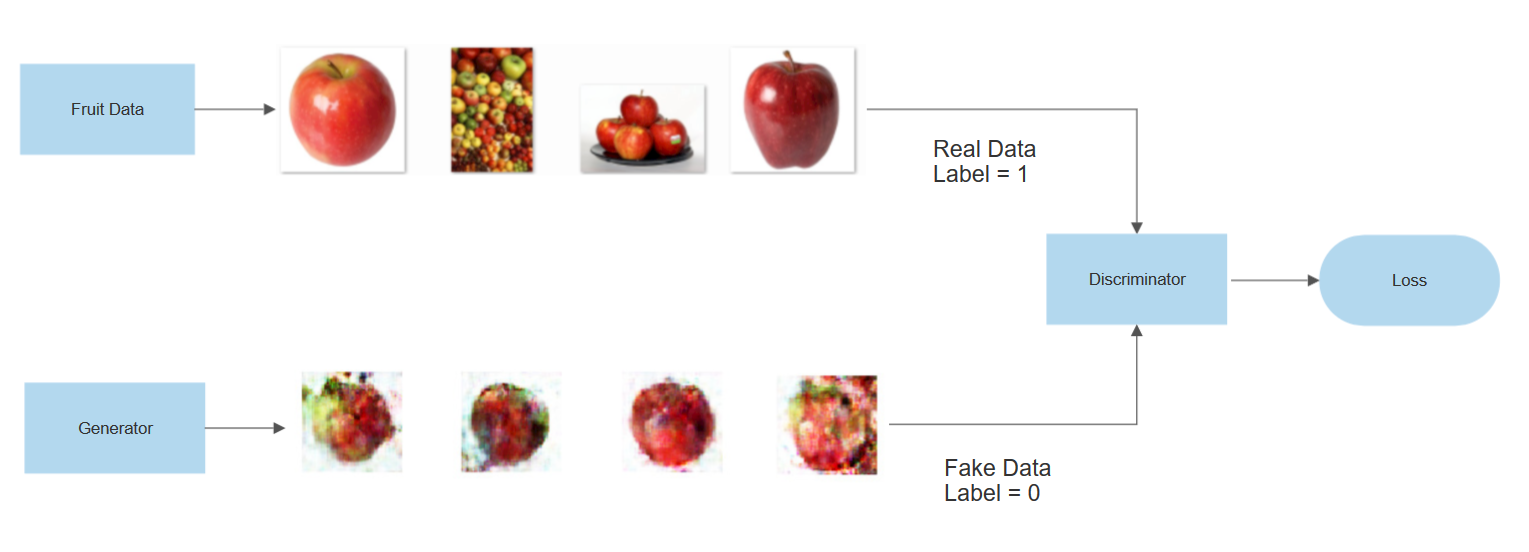
\includegraphics[width=\textwidth]{models/training_discriminator.png}}
\caption{Discriminator Training with real and generated data}
\label{fig:train_discriminator}
\end{figure}

After that the weights of the Discriminator are frozen, and the output of the Generator is linked to the input of the Discriminator. The input, a random noise vector, is then fed into the Generator and the produced images are labelled with 1. Each image, which the Discriminator recognises as being fake, results in an immediate loss for the Generator. Because the weights of the Discriminator are frozen, only the Generator learns to generate better images and the Discriminator is not affected negatively. This is summarised in Figure \ref{fig:train_generator}.

% After that we train our Generator by creating fake data and labelling them as true (label = 1), trying to fool the Discriminator and using the loss to update our model.
\begin{figure}
\centering
\centerline{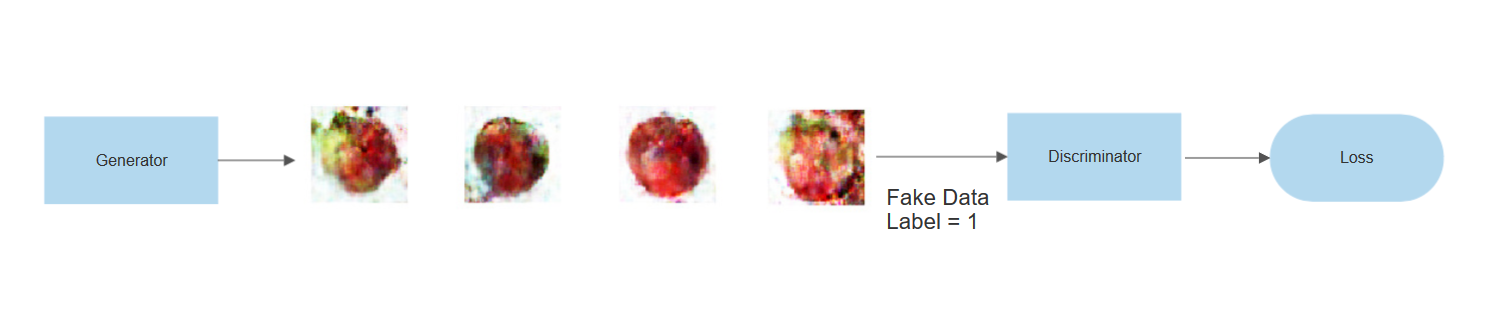
\includegraphics[width=\textwidth]{models/training_generator.png}}
\caption{Overview of the Generator Training Structure}
\label{fig:train_generator}
\end{figure}

Doing these processes repeatedly we are able to train our Discriminator and our Generator. The better one network gets, the better the other network gets (under good parameter settings).

Compared to the normal approach of training a GAN, where all classes of a dataset are used at once, we train one GAN model for each class. This is necessary due to the fact that we need to label the produced images according to the class they try to replicate.

\subsection{Models}
Both, the Discriminator as well as the Generator, use a Deep Neural Network.
For the Discriminator, we first started with a sequential network consisting of four Convolutional2D layers, which used LeakyReLU with an alpha of 0.2 as the activation function. Each convolutional layer is followed by a dropout layer with a dropout rate of 0.4.
Finally, the output is flattened and used as input for a dense layer, which used Sigmoid as the activation function to predict a single value between 0 and 1 as the probability of an image being real.

The Generator also consisted of a sequential network, where the input was a random noise vector with a length of 100.
A dense layer with ReLU uses the noise and is followed by a reshaping layer, which reshapes the input to a 16 x 16 x 128 matrix.
After that we used a combination of batch normalization with a 0.9 momentum, dropout with 0.4, up-sampling layers, and convolutional layers. All but the last layer used ReLu as the activation function. The final layer used Sigmoid again. For the optimization of both models we used Adam with a learning rate of 0.0002, beta one with 0.5, and beta two with 0.999. We noted that a very small learning rate is quite important for GAN's. Having a too high learning rate resulted in images which were impossible to recognise.

We then tried to reduce the noise by varying the dropout rate and using LeakyReLU in the Discriminator with an alpha of 0.2 as well. For the Generator we only changed the last activation function to the tangens hyperbolicus. This provided good results, however the loss of the Discriminator quickly converged which made it difficult for the Generator to learn. Thus we changed the optimizer to use RMSProp with different learning rates to tackle this effect. We used a learning rate of 0.0004 with a decay of 3e-8 for the Generator and 0.0008 with a decay of 6e-8 for the Discriminator. This still did not improve the network too much so we changed back to Adam.

\begin{figure}[h!]
\centering
\centerline{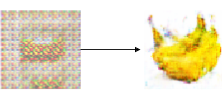
\includegraphics[width=0.5\textwidth]{plots/tuning.png}}
\caption{Change of the image quality through hyper parameter tuning}
\label{fig:tuning}
\end{figure}


Afterwards, we tried out the idea of training the Discriminator additionally during the training of the Generator, which proved similar results. Since the images were still not satisfying, and to prove the functionality of our GAN, we gathered more training data, in this case of bananas, which improved the quality of the images.

The final model of the Generator is shown in Figure \ref{fig:generator} and the final model of the Discriminator is shown in Figure \ref{fig:discriminator}. The results of our parameter tuning can be seen in Figure \ref{fig:tuning}.

% model explanation
% model pictures



\section{Evaluation}
The task of this exercise was to see how well a classifier works with different training data, but same test data. 
As mentioned in Section \ref{sec:introduction} we trained 3 different classifiers. The first was trained on original training data, the second was trained on simulated data and the third was trained on synthetic data, that was generated with our in Section \ref{sec:gan} explained GAN. This process can be seen in Figure \ref{fig:cnn_evaluation}.

For the construction of our simulated data we have used the following operations:
\begin{itemize} 
    \item horizontal flipping
    \item brightness adjustment in the range [0.2, 1.0]
    \item picture zooming in the range [0.5, 1.0] 
    \item picture rotation in the range [-25$^{\circ}$, +25$^{\circ}$]
\end{itemize}

% CNNs
For the CNN we have used a simple Convolutional Neural Network consisting of five Convolutional and MaxPooling Layers.
After that we flatten it, use dropout and then apply two Dense Layers. Our CNN can be seen in Figure \ref{wrap-fig:cnn}.

% Evaluation
\begin{figure}[h!]
\centering
\centerline{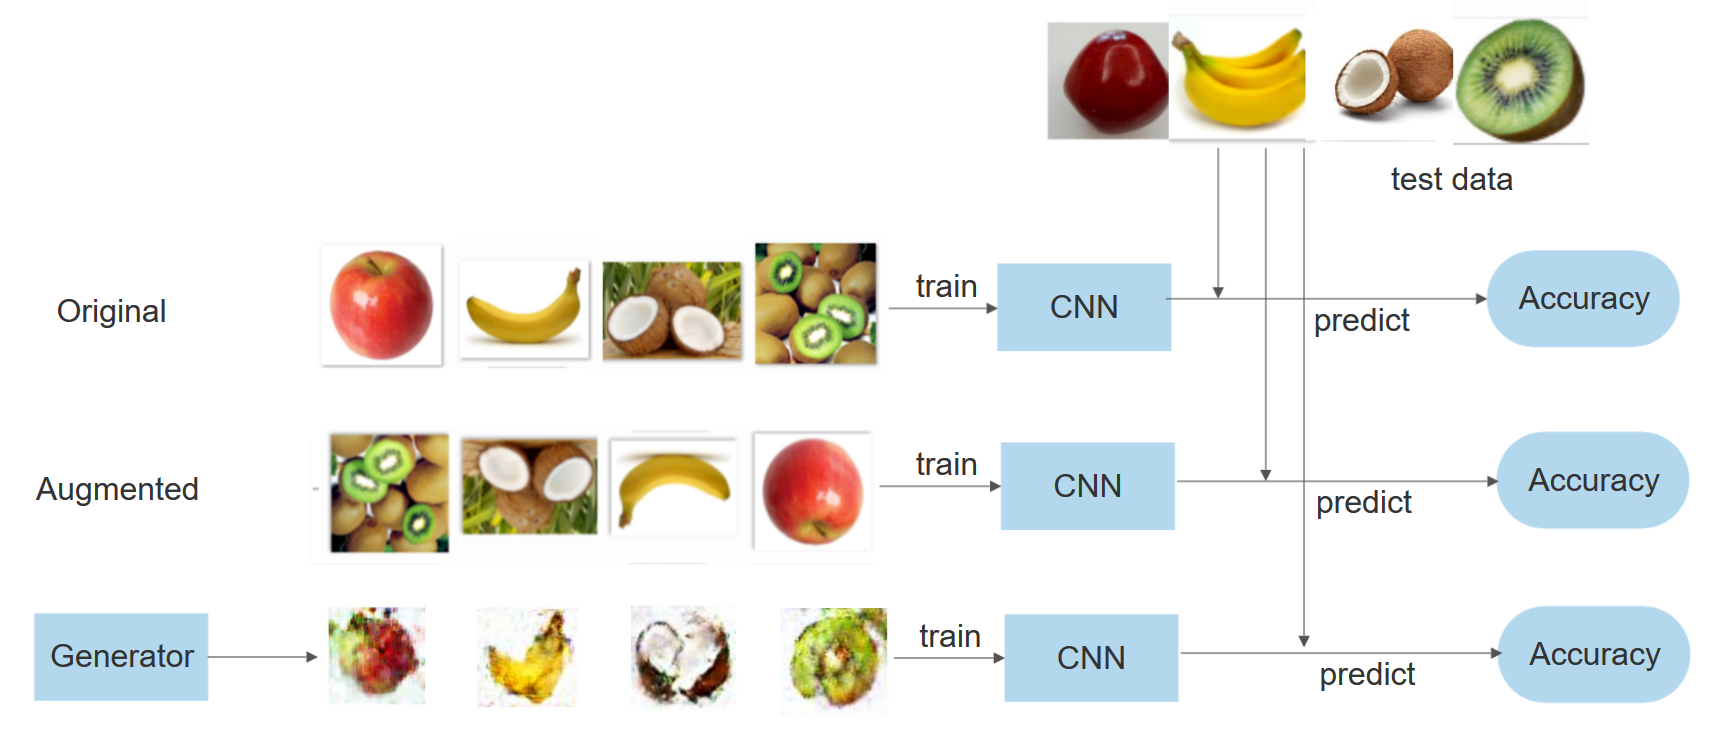
\includegraphics[width=\textwidth]{models/evaluation_CNN_comparison.png}}
\caption{Overview of program pipeline}
\label{fig:cnn_evaluation}
\end{figure}
\newpage
\section{MNIST dataset}
We have decided on trying out our Generator on a simple dataset which contains a lot more training samples.
MNIST proves interesting, as the pictures offer less sophisticated features which are mostly just simple edges and lines.
Our MNIST dataset contains 42k pictures, with 4k instances for each of the ten classes [0-9]. 
We wanted to see how this effects the generation; thus we have trained a GAN for 30 epochs per class with a batch size of 128. 
In Figure \ref{fig:generated_numbers} the results of each GAN [epoch 30] can be seen.

\begin{figure}[h!]
\centering
\centerline{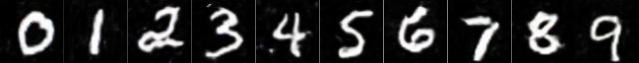
\includegraphics[width=\textwidth]{plots/numbers.png}}
\caption{Generated pictures from MNIST dataset}
\label{fig:generated_numbers}
\end{figure}

For the evaluation we have generated 8k images per class using the model from the 30th epoch or rather the last model from training.
Looking at the generated data, we see that while some classes seem to perform marginally better than others, we still are able to generate perfectly valid numbers for every class as seen in Figure \ref{fig:generated_numbers}. However even during later epochs some faulty generations happen which can be seen in Figure \ref{fig:generated_numbers_bad}.

\begin{figure}[h!]
\centering
\centerline{
\includegraphics[width=0.3\textwidth]{plots/numbers_bad_generation.png}}
\caption{Good generation versus bad generation of number 2 from MNIST dataset}
\label{fig:generated_numbers_bad}
\end{figure}

Analysing the validation loss in figure \ref{fig:generated_numbers_loss}, we can see that the Generator loss jumps up to 2.5, because the Discriminator gets better at distinguishing real and fake data. However after 1000 episodes the loss converges to around 1, while the Discriminator loss starts low and increases over time until it converges at around 0.8. After these 400 iterations it can also be seen that the accuracy of the Discriminator seems to oscillate around 50 \%, which means that on average it cannot distinguish between a real and a fake image anymore.

\begin{figure}[h!]
\centering
\centerline{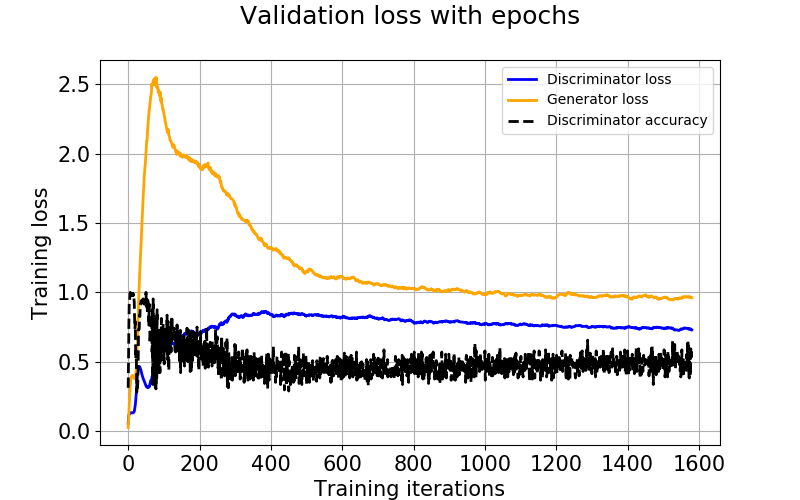
\includegraphics[width=0.58\textwidth]{plots/mnist/0_loss.png}}
\caption{Discriminator - Generator loss after time}
\label{fig:generated_numbers_loss}
\end{figure}
% pic val loss
\newpage
Looking at the training accuracy and training loss, in Figures \ref{fig:mnist_training}, \ref{fig:mnist_validation}, we see that the CNN trained with fake data performed best, while the CNN trained with augmented data performed worst. As can be seen in the validation plots however, the CNN trained on generated data did not perform as well as the one trained on actual data; the augmented CNN being in the middle. This could be explained due to the fact that our original dataset is big enough and the CNN learns more sophisticated features the closer the data is to being original. While the CNN trained with synthetic data seems to get worse after a few epochs, the other ones benefit from longer training. All in all, they still perform quite similarly and the difference between them is around 3 percent.
% conclusio dataset
\begin{figure}[h!]
    \centering
    \begin{subfigure}[b]{0.48\textwidth}
        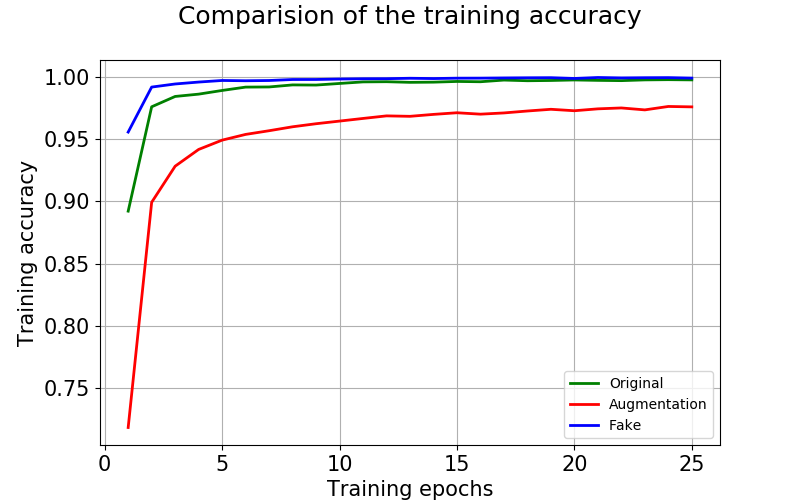
\includegraphics[width=\textwidth]{plots/mnist/comparision_acc.png}
        \caption{Training accuracy}
    \end{subfigure}
    ~ 
    \begin{subfigure}[b]{0.48\textwidth}
        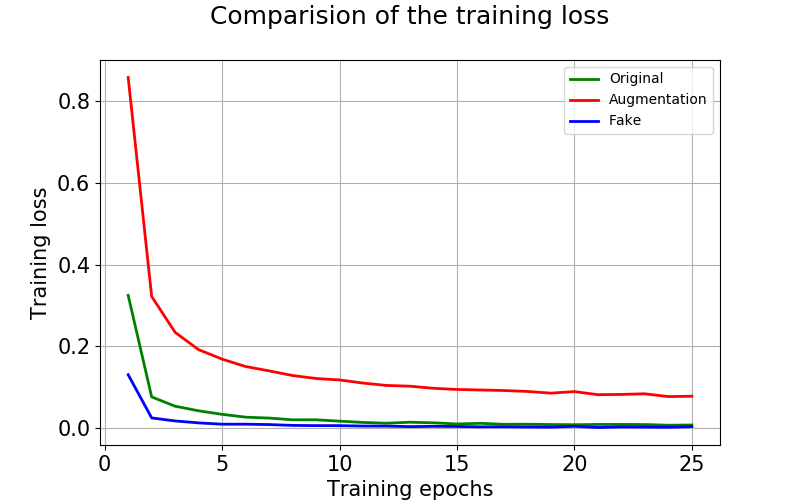
\includegraphics[width=\textwidth]{plots/mnist/comparision_loss.png}
        \caption{Training loss}
    \end{subfigure}
    \caption{Overview of the loss and accuracy of the training}
    \label{fig:mnist_training}
\end{figure}

\begin{figure}[h!]
    \centering
    \begin{subfigure}[b]{0.48\textwidth}
        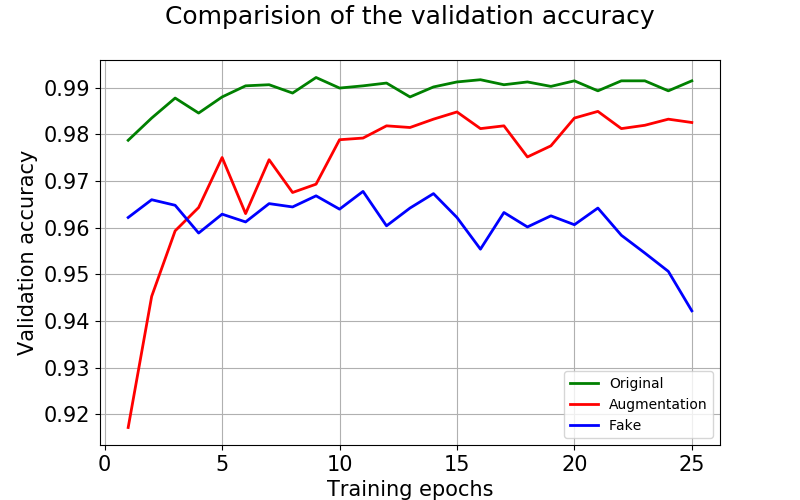
\includegraphics[width=\textwidth]{plots/mnist/comparision_val_acc.png}
        \caption{Validation accuracy}
    \end{subfigure}
    ~ 
    \begin{subfigure}[b]{0.48\textwidth}
        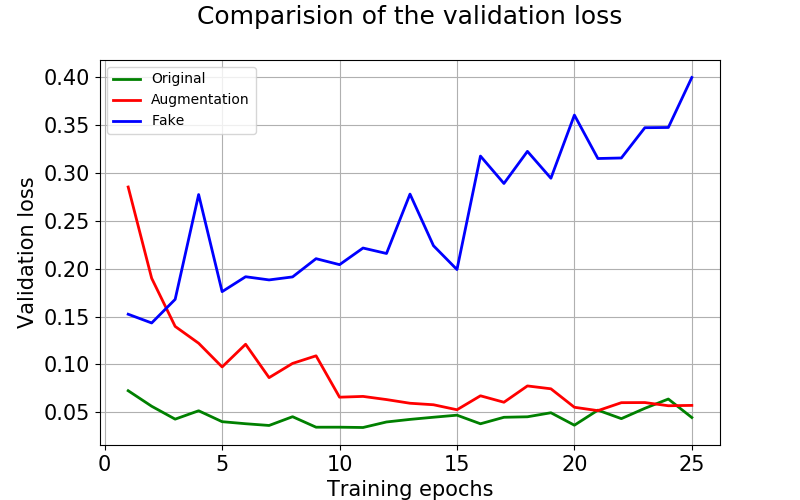
\includegraphics[width=\textwidth]{plots/mnist/comparision_val_loss.png}
        \caption{Validation loss}
    \end{subfigure}
    \caption{Overview of the loss and accuracy of the validation}
    \label{fig:mnist_validation}
\end{figure}


\section{FIDS30 dataset}\label{FIDS30}
For our next dataset we have decided on tackling the problem from another side, trying to generate pictures based on a low amount of input data; this time also with color. Therefore we picked ten different fruits for which we generated synthetic data. Because the amount of training data was so little, average of 35 images per class, we trained our GANs for each fruit for 1000 epochs with a batch size of 6.

For the selection we tried to choose fruits with very different characteristics on shape and color. The chosen fruits can be observed in Table \ref{tab:fruits}.

After we split the dataset in 80 \% training and 20 \% validation and trained the multiple GANs, we chose for each class the model which produced the best looking, and most realistic images. The exact epoch for each fruit can also be observed in Table \ref{tab:fruits}. Unfortunately the loss of the Generator, in opposition to the one for the MNIST dataset, did not converge. This can also be seen when the generated images are observed (Figure \ref{fig:genfruits}) as they contain a lot more noise. 

\begin{table}[h]
    \centering
    \begin{tabular}{|l|c|}
    \hline
        Class & Epoch \\ \hline
        Strawberries & 390 \\ \hline
Raspberries & 630 \\ \hline
Limes & 870 \\ \hline
Kiwifruits & 690 \\ \hline
Grapes & 360 \\ \hline
Coconuts & 990 \\ \hline
Blueberries & 690 \\ \hline
Bananas & 420 \\ \hline
Apricots & 690 \\ \hline
Apples & 570 \\ \hline
    \end{tabular}
    \caption{Selected fruits with the chosen epoch for image generation}
    \label{tab:fruits}
\end{table}

For each class we then generated 600 images, especially to tackle the problem of our original training set being too small. We then evaluated the real, augmented and the synthetically generated data with our previously mentioned classifier over 48 epochs with a batch size of 12.

\begin{figure}[h!]
\centering
\centerline{
\includegraphics[width=\textwidth]{plots/fruits.png}}
\caption{Strawberries, raspberries, limes, kiwifruits, grapes, coconuts, blueberries, bananas, apricots, and apples generated by the Generator}
\label{fig:genfruits}
\end{figure}

Comparing the results of Figure \ref{fruits_training}, we can clearly observe that the synthetic data converged the fastest during training. After 40 epochs the real data reached the same accuracy and loss as the generated data. However, the augmented data performed 20 \% worse, archiving only 80 \% accuracy, whereas the real and the generated data reached 100 \%. The reason behind the bad performance of the augmented data might be that varying all those parameters, results in a much wider space of possibilities and thus in endless different images, which is very hard to learn.

\begin{figure}[h!]
    \centering
    \begin{subfigure}[b]{0.48\textwidth}
        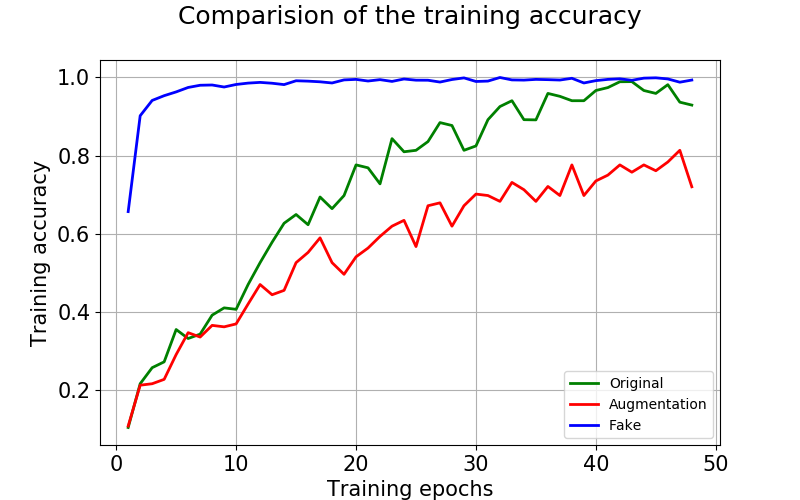
\includegraphics[width=\textwidth]{plots/fruits/comparision_acc.png}
        \caption{Training accuracy}
    \end{subfigure}
    ~ 
    \begin{subfigure}[b]{0.48\textwidth}
        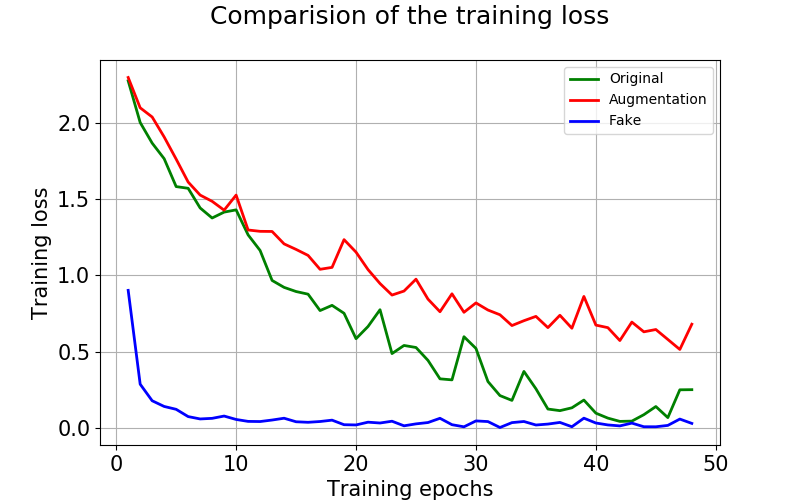
\includegraphics[width=\textwidth]{plots/fruits/comparision_loss.png}
        \caption{Training loss}
    \end{subfigure}
    \caption{Overview of the loss and accuracy of the training}
    \label{fruits_training}
\end{figure}

Comparing the performance on the unseen validation set for each episode in Figure \ref{fruits_validation}, we observed that the synthetic generated data reached a 65 \% accuracy the fastest. This already happened for the fake data in epoch 1. Concerning the real and the augmented data, they only reach this level of performance at around epoch 15. This clearly shows that using synthetic generated data speeds up the training process quite significantly. However, we should not forget that it also takes a lot of time to generate those images in the first place. Lastly, we want to add that the model on the generated data over fits early on, resulting in a much higher loss.

\begin{figure}[h!]
    \centering
    \begin{subfigure}[b]{0.48\textwidth}
        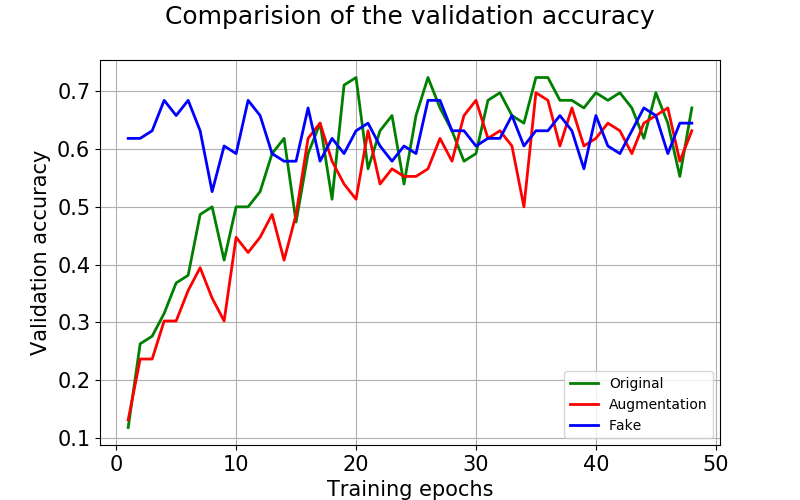
\includegraphics[width=\textwidth]{plots/fruits/comparision_val_acc.png}
        \caption{Validation accuracy}
    \end{subfigure}
    ~ 
    \begin{subfigure}[b]{0.48\textwidth}
        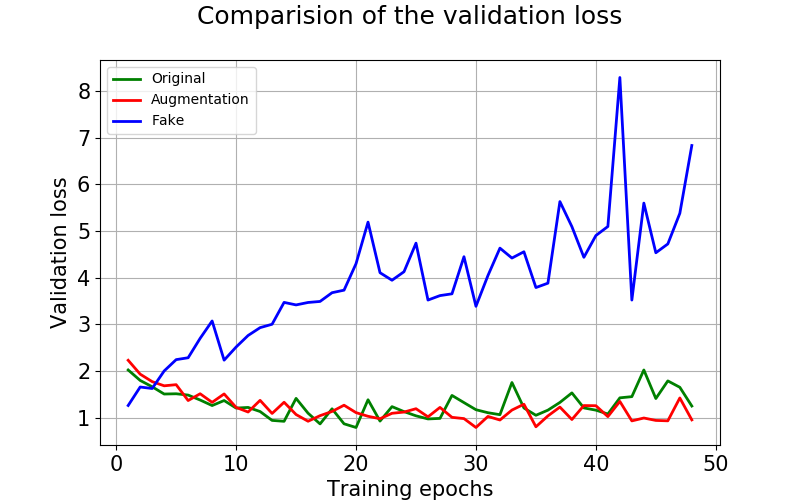
\includegraphics[width=\textwidth]{plots/fruits/comparision_val_loss.png}
        \caption{Validation loss}
    \end{subfigure}
    \caption{Overview of the loss and accuracy of the validation}
    \label{fruits_validation}
\end{figure}


% parameters / approaches tried

% results
    % some colours were better etc

% conclusio dataset

\section{Conclusion}

Looking at the plots of the MNIST dataset, we can see that the networks seem to converge to a point where the Discriminator is not able to distinguish between an original and a generated picture and thus can only guess which explains the accuracy of around 50 \%. However, this is not the case for the FIDS30 dataset, where the Discriminator outperforms the Generator substantially. Important to mention is that the generated pictures still exhibit a lot of noise which makes them look synthetic, and thus makes them easily
classifiable to the human eye, whereas this is not the case for images generated for the MNIST dataset.

\begin{figure}[h!]
    \centering
    \begin{subfigure}[c]{0.48\textwidth}
    \centering
        
\includegraphics[width=0.6\textwidth]{plots/comparison_fruits.png}
        \caption{Synthetic Coconut vs Real Coconut}
    \end{subfigure}
    ~ 
    \begin{subfigure}[c]{0.48\textwidth}
    \centering
        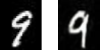
\includegraphics[width=0.6\textwidth]{plots/comparison_mnist.png}
        \caption{Synthetic 9 vs Real 9}
    \end{subfigure}
    \caption{Overview of the generated image quality}
    \label{fig:quality}
\end{figure}

Despite the fact that the generated images were clearly distinguishable for the fruits dataset, the CNN classification performance on the validation set was about as good for the CNN trained on synthetic data as the one trained on original data; with the fake trained one even having a higher accuracy during the first training rounds. However, after the evaluation, the models trained on the fake data were also the models with the highest loss and thus with the worst accuracy, which can be interpreted in the way that those models over-fitted to the low level features of the synthetic data.

Concerning our GANs and their performance, we conclude that obviously it is much easier for the Generator to fool the Discriminator when dealing with data which has only one colour channel and are high in contrast. This is the case on the MNIST dataset where we only have greyscale images with a high contrast. Compared to that, on the FIDS30 dataset, images with 3 colour channels and a very different structure between the images have to be learned.

Even though the synthetic images do not look realistic, the GANs were still be able to pick up the key characteristics such as colour and form of a fruit or a digit. This phenomena can be observed in the evaluation process: the previously extracted characteristics of the GANs' created images result in a much faster ability to correctly classify the validation set. This also explains why the accuracy drops after a while, since it tries to find and learn more hidden meaning behind the underlying structure of the generated images, which does not exist within the fake data, since the Generator is not that good.

Observing CNNs trained on augmented data, concerning the trained models and their performance on the validation set, they are just slightly below the models trained on the real data. The real difference between them is only noticeable in the training accuracy, since most of the times their performance is significantly lower then the generated and real data. As mentioned in Section \ref{FIDS30}, this might be the case due to the endless possibilities augmentation offers and therefor it is especially hard for the model to learn those small differences.

To conclude, synthetic generated data can work well to get a good initial prediction very fast but also over-fits earlier than usual approaches like augmentation and using real data. Thus one needs to evaluate what takes more time: to train multiple GANs and to generate synthetic data or to train the CNN with real data.

\begin{figure}
    \centering
    \begin{subfigure}[b]{0.36\textwidth}
        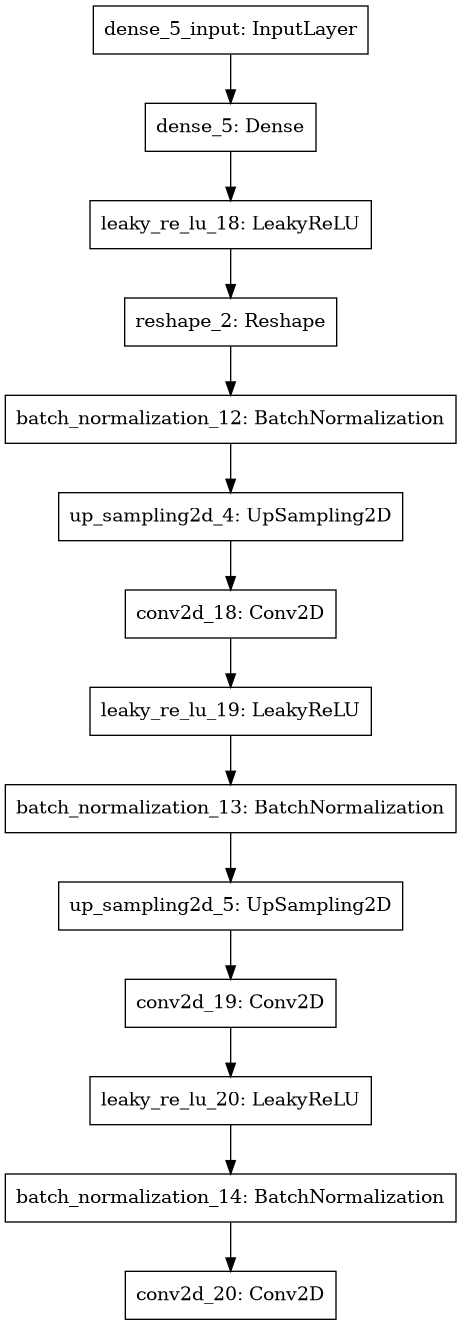
\includegraphics[width=\textwidth]{plots/generator.png}
        \caption{Generator}
        \label{fig:generator}
    \end{subfigure}
    \hspace{3cm}
    \begin{subfigure}[b]{0.36\textwidth}
        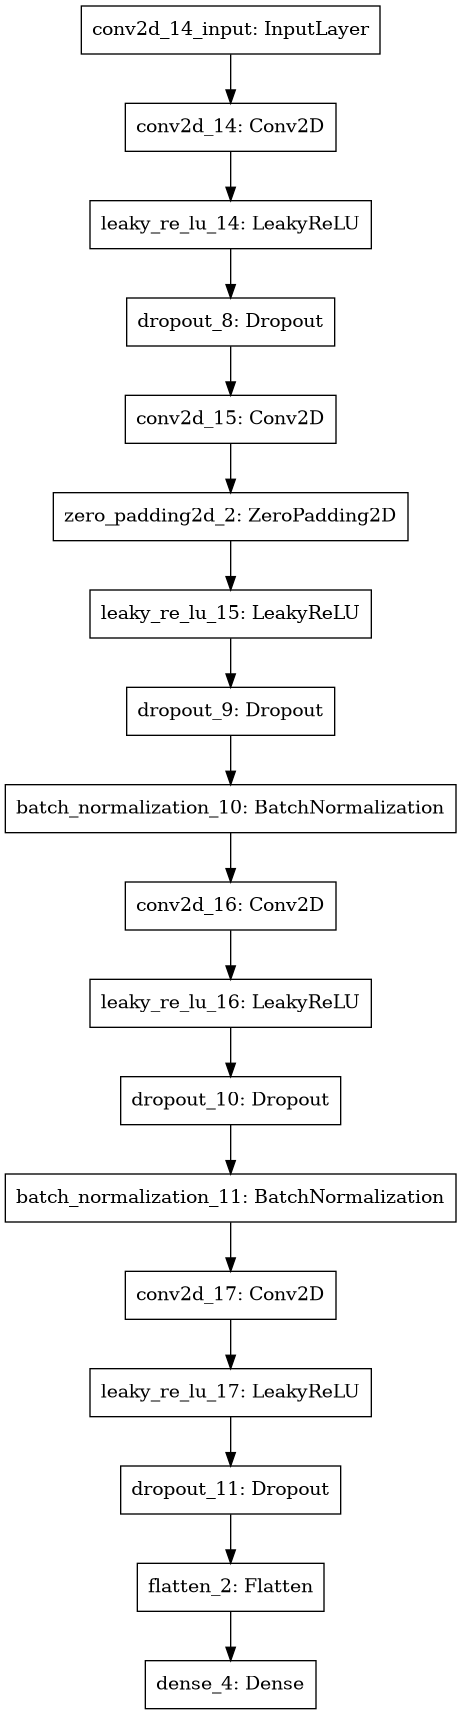
\includegraphics[width=\textwidth]{plots/discriminator.png}
        \caption{Discriminator}
        \label{fig:discriminator}
    \end{subfigure}
    \vspace{5mm}
    \caption{Overview of the models used in the GAN}
\end{figure}


\begin{figure}
\centering
\centerline{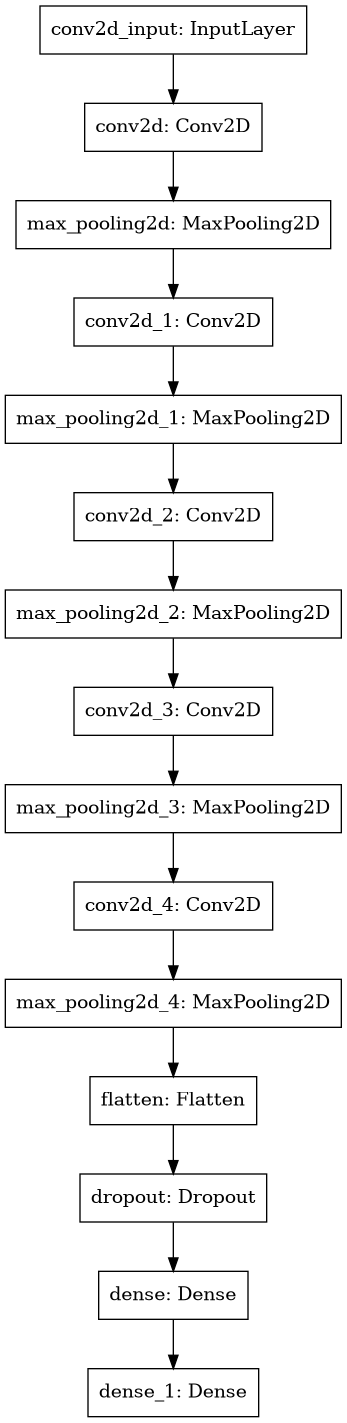
\includegraphics[width=4.5cm]{plots/cnn.png}}
    \vspace{5mm}
\caption{Convolutional Neural Network structure for the evaluation}\label{wrap-fig:cnn}
\end{figure}

\end{document}


